\chapter{Local polynomial regression}
\section{Different bandwidths and kernels}
This exercise is about a method for non-parametric regression called local polynomial regression (LPR). It is a generalisation of the kernel based Nadaraya-Watson estimator, similar to the kernel density estimation in Exercise 6. The Nadaraya-Watson estimator is a local weighted mean estimation. The local polynomial regression estimation for $(X_1,Y_1),...,(X_n,Y_n)\stackrel{iid}{\sim}(X,Y)$ and the model $$Y_i=f(X_i)+\varepsilon_i, \; \varepsilon_i \stackrel{iid}{\sim}\left\langle0,\sigma^2\right\rangle$$ is derived by a Taylor approximation of the function $f$. 
\begin{figure}[!htb]
\centering
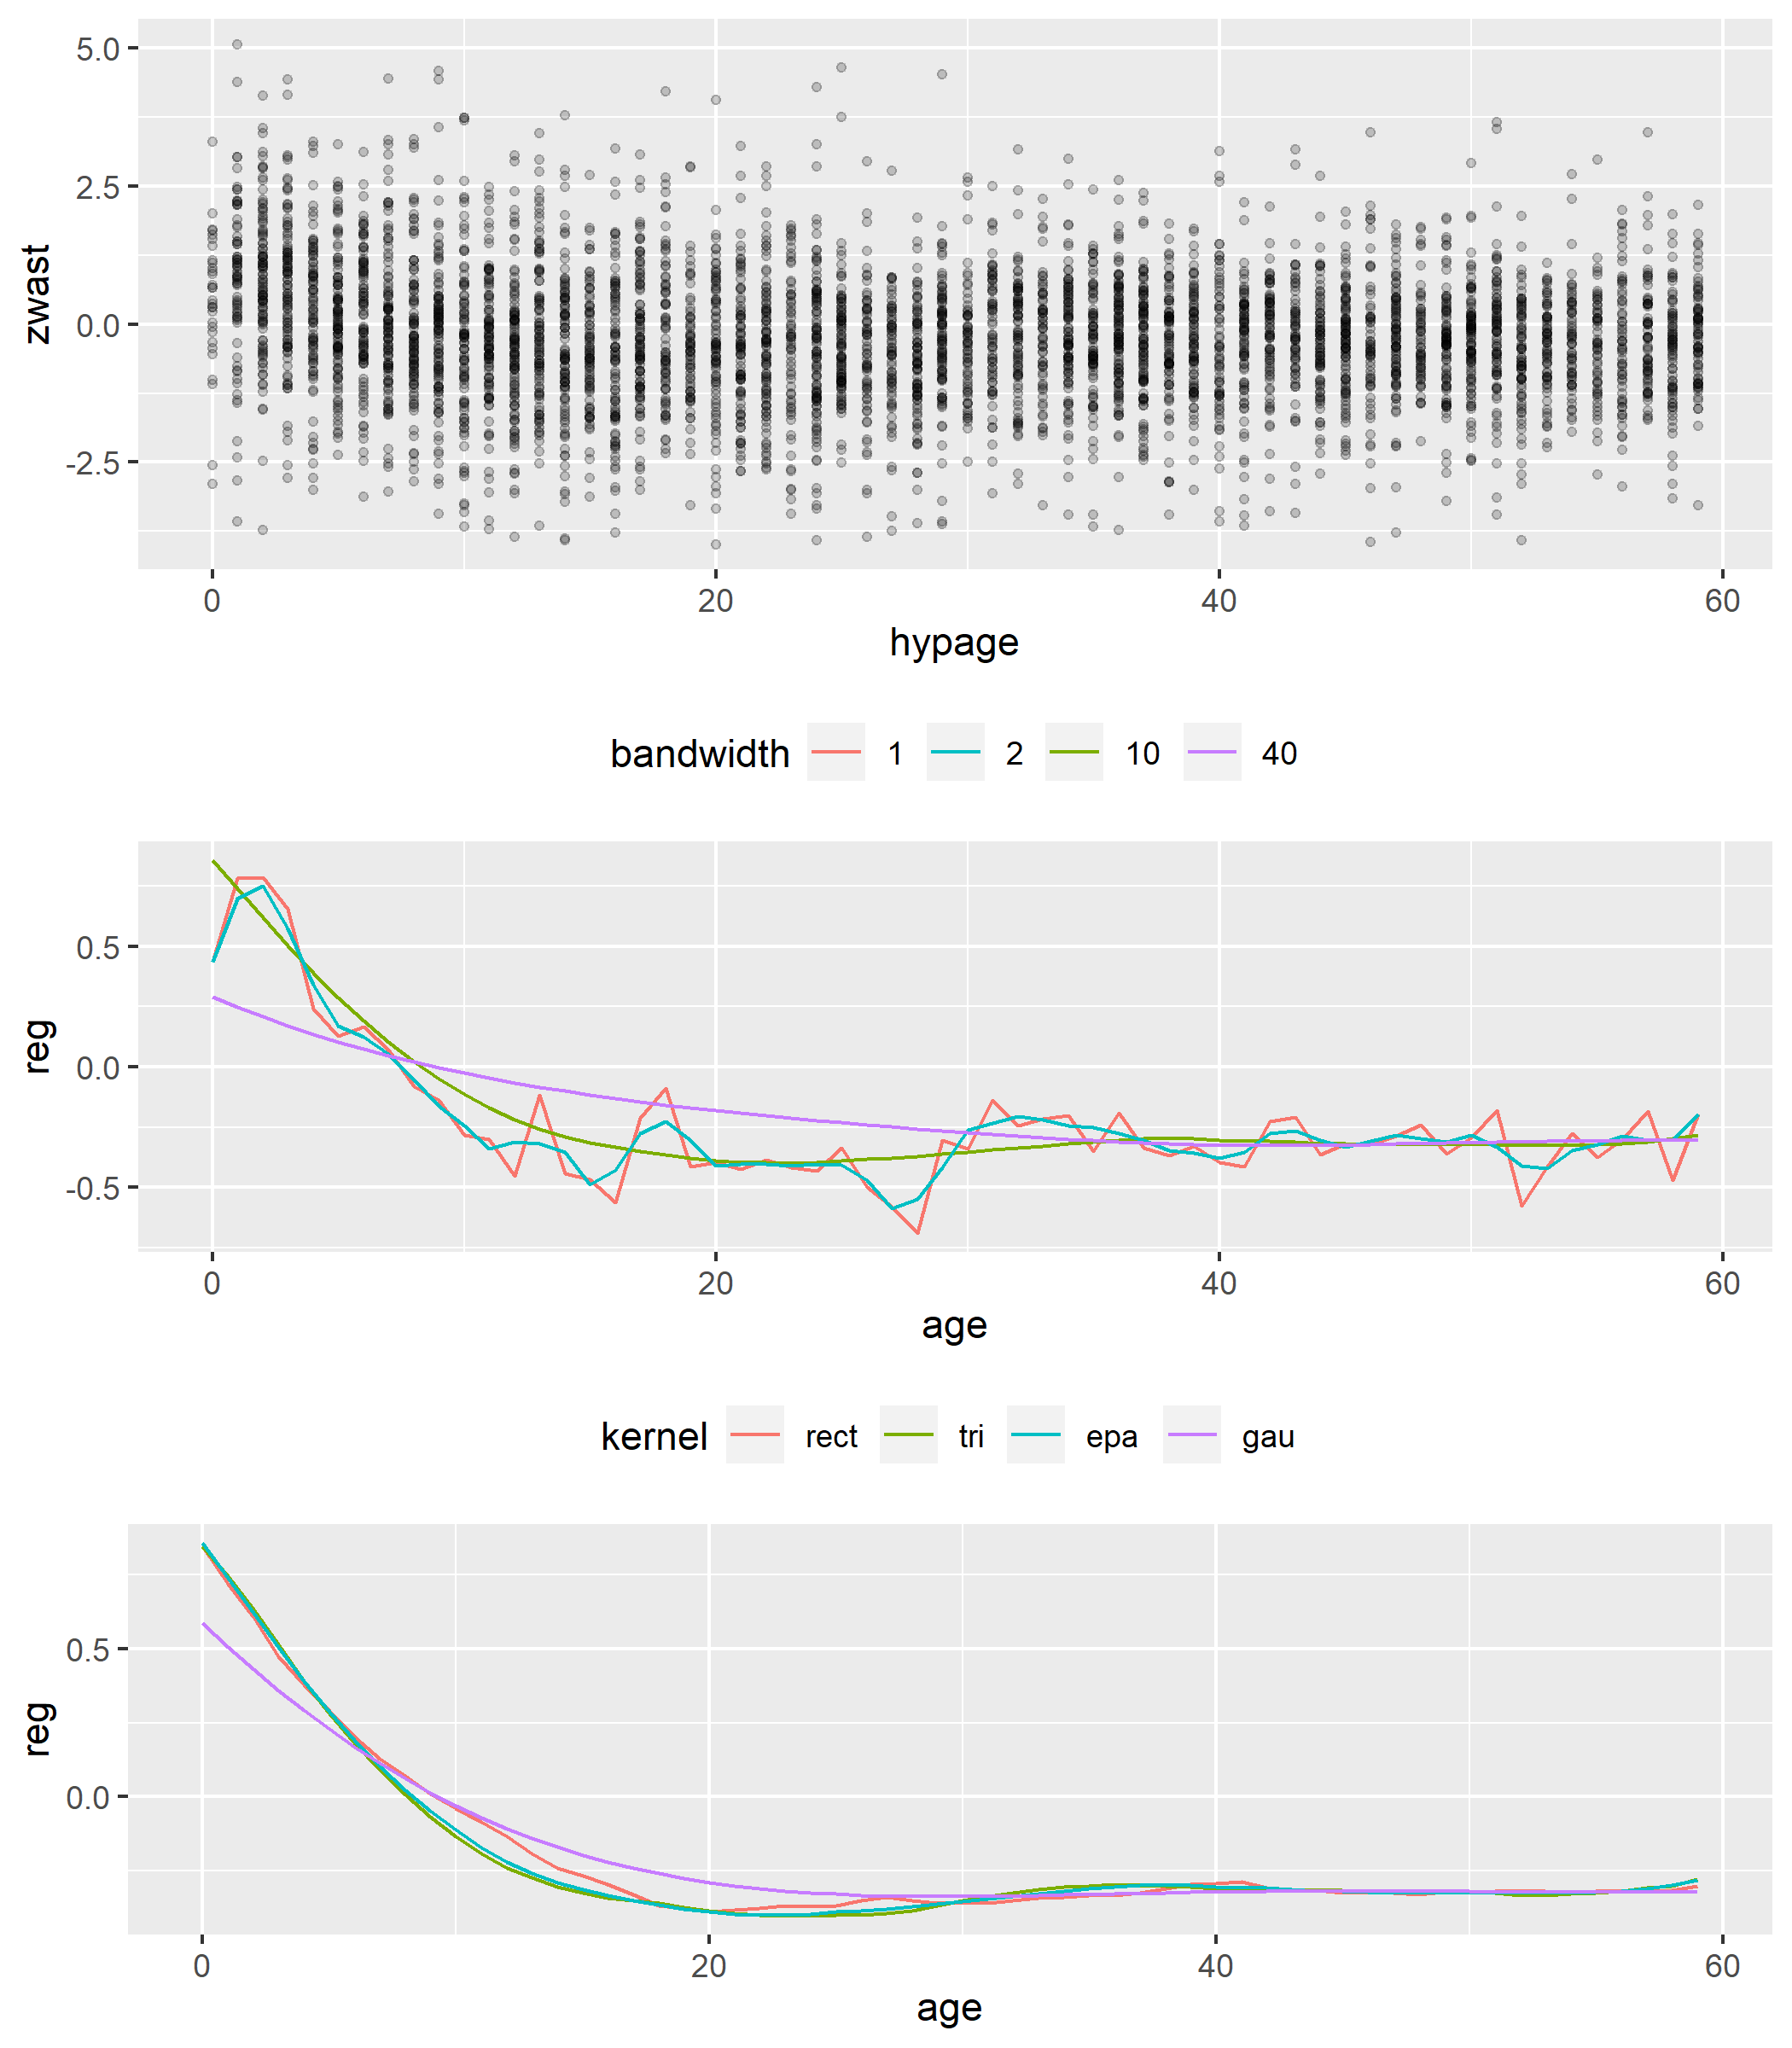
\includegraphics[width=0.8\textwidth, keepaspectratio]{ex9/polyfits.png}
\caption{First: Age against Z-score in the Kenyan children data. Second row: LPR fit with different bandwidths and Epanechnikov kernel. Third: LPR fit with different kernels and fixed bandwidth $h=10$.}
\label{7fits}
\end{figure}

We apply this method to the data of Kenyan children already used in Exercise 1. We want to fit a curve for the Z-score for wasting (\texttt{zwast}) against age. This Z-score is a transformation of a child's weight standardised by the median and standard deviation of the weight of healthy children with the same height. We wrote our own function for fitting a local polynomial curve with data, bandwidth, kernel and polynomial order as arguments. To examine the influence of argument choice we again fitted a curve for different bandwidths and the same kernels as in Exercise 6 with a fixed order 1 polynomial regression (see Figure \ref{7fits}).

We see similar results as in Exercise 6. With increasing bandwidth the curve gets smoother. With a bandwidth of 1 the fit represents the data rather locally. With $h=2$ some of the fluctuations are flattened out and with increasing bandwidth the curve converges to the constant mean of the data (see blue line). I took 40 as the highest bandwidth here to demonstrate this fact. A reasonable choice seems to be $h=10$ since there the functions looks pretty smooth but still represents the first drop of the Z-score and the slight increase and convergence afterwards that we see in the scatter plot in Figure \ref{7fits}. Then using this bandwidth we were asked to fit the curve for different kernels. Like in Exercise 6 again we see that the Gaussian kernel produces the most flat curve. Indeed it looks quite similar to the fit for the Epanechnikov kernel with an astonishing high bandwidth compared to the one used here. The fits for the triangular and Epanechnikov kernel don't differ obviously. The red line representing the fit for the rectangular kernel seems piecewise linear which is quite natural as the kernel is piecewise constant and we used a LPR of order 1 (i.e. using linear polynomials) in all these plots.  

\section{Generalised cross-validation}
Similar to the cross-validation method in Exercise 6 there is a generalised version for LPR we want to use here to find the best bandwidth for different polynomial degrees. The generalised cross-validation criterion (GCV) is given by $$GCV(h)=\frac{\sum_{i=1}^{n}{\left[Y_i-\hat{f}_{n,h}(X_i)\right]^2}}{1-n^{-1}\sum_{i=1}^{n} W_{i}(X_i,h)}$$ where $W_i$ are the weights of the different observations for the linear generalised least square estimation used to compute the parameters. This time we used only the Epanechnikov kernel to search for the minimal GCV. Again we have the same problem - like in Exercise 6 - that the GCV curve is not unimodal and thus optimize won't find the global minimum (see Figure \ref{7opth}). 
\begin{figure}[!bht]
\centering
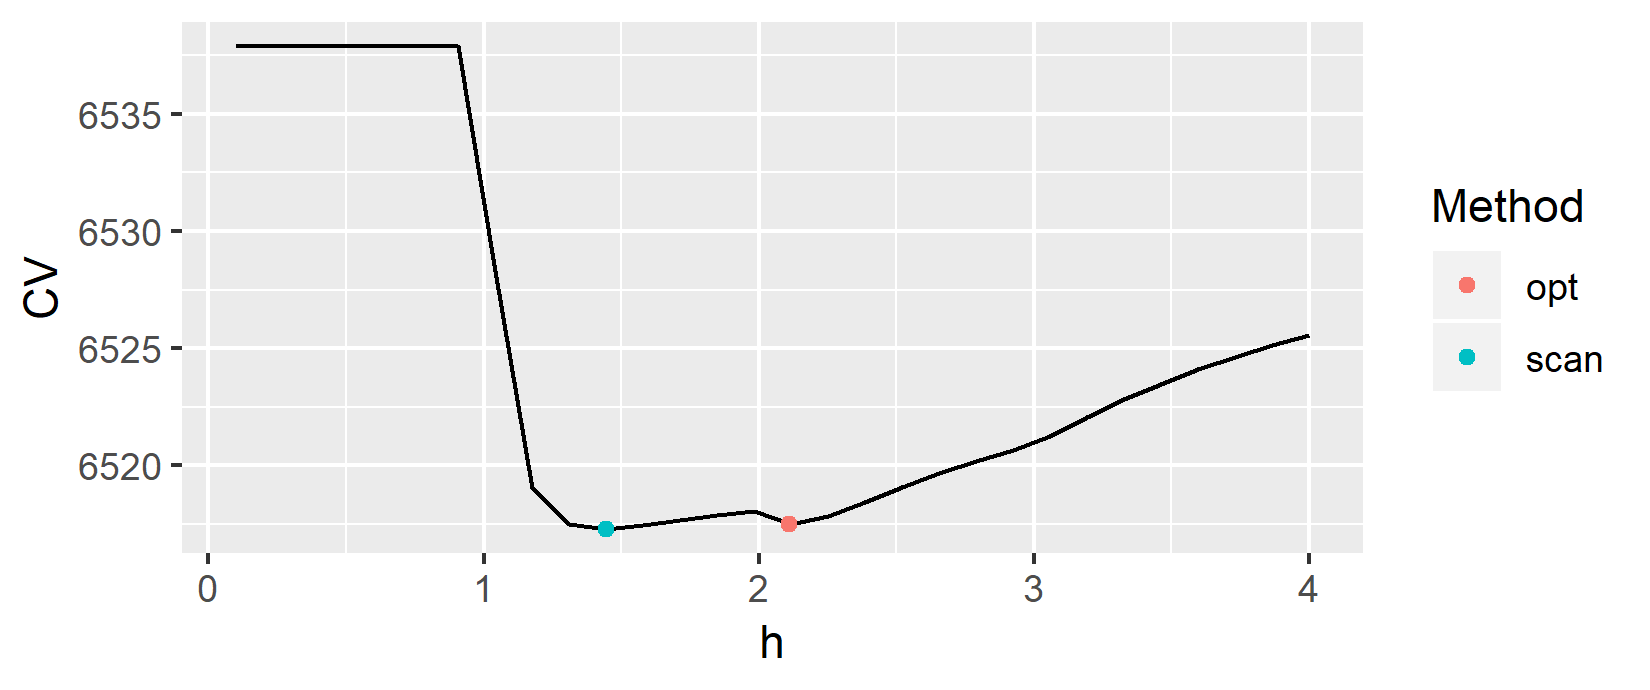
\includegraphics[width=0.8\textwidth, keepaspectratio]{ex9/opth.png}
\caption{GCV against $h$. Points show optimal $h$ for the scan over 30 points (blue) and the \texttt{optimize} function (red).}
\label{7opth}
\end{figure}

We therefore use a scanning strategy only to get the optimal bandwidths. The results are shown in Table \ref{7tableh}. We see that the results for degree 2 and 3 are identical (rounded to two digits) and similar to the results for degree 4 whereas for degree 1 a lower bandwidths seems the best option. The degree 4 fit gives the highest GCV indicating a worse fit.
\begin{table}[!ht]
\centering
\begin{tabular}{lrr}
  \hline
deg & h & GCV \\ 
  \hline
1 & 1.44 & 6517.30 \\ 
  2 & 3.19 & 6518.00 \\ 
  3 & 3.19 & 6518.00 \\ 
  4 & 3.06 & 6522.78 \\ 
   \hline
\end{tabular}
\caption{Optimal bandwidth $h$ together with minimal GCV for different polynmial degrees (deg).}
\label{7tableh}
\end{table}

Now have a look at the fitted curves (see Figure \ref{7fitsh}). The curves don't differ but look very similar. This is especially surprising since the optimal bandwidth for degree 1 is much lower than for the other curves. But with higher polynomial degree the regression as more degrees of freedom (i.e. more parameters) to adapt to the data. This would explain why all three curves look like a very local fit. On the left border all three curves decrease as age tends to 0. This does not seem reasonable since the shape of the data suggests that the Z-score is very high at birth and decreases rapidly in the first months. This is one disadvantage of local non-parametric regressions, that in general at the border and outside of the observed data range the prediction is not valid and thus generalisations difficult. Finally note, that the curves in Figure \ref{7fitsh} look piecewise linear. Indeed in this plot they are drawn since we approximated the regression curves at the data points. One could have generalised the function fitting the curve with an argument $x$ to draw a better approximation with more points but note that one has to fit a linear model for every point then and this would lead to higher computational effort. Still one would recognizes difference in shape in the way the data is presented here. Summing up and looking back to the second plot in Figure \ref{7fits} using the GCV may not be the best method to find a suitable bandwidth in every case but can result in a - in my opinion - too low bandwidth that results in a more local representation than a reasonable and useful trend analysis of the data.   

\begin{figure}[!t]
\centering

\includegraphics[width=0.8\textwidth, keepaspectratio]{ex9/fitsh.png}
\caption{LPR fit for different polynomial degrees each with optimal bandwidth according to Table \ref{7tableh} with Epanechnikov kernel.}
\label{7fitsh}
\end{figure}

\section{Estimating derivatives}
When considering the change of a variable over time it may be useful to have a look at the derivative of the curve. The method of LPR provides also an on-the-fly method to estimate the derivatives since it is based on a Taylor expansion of the function. For a regression of the derivatives of the curve we use the R function \texttt{localpoly.reg} in the package \texttt{NonpModelCheck}. 
\begin{figure}[p]
\centering
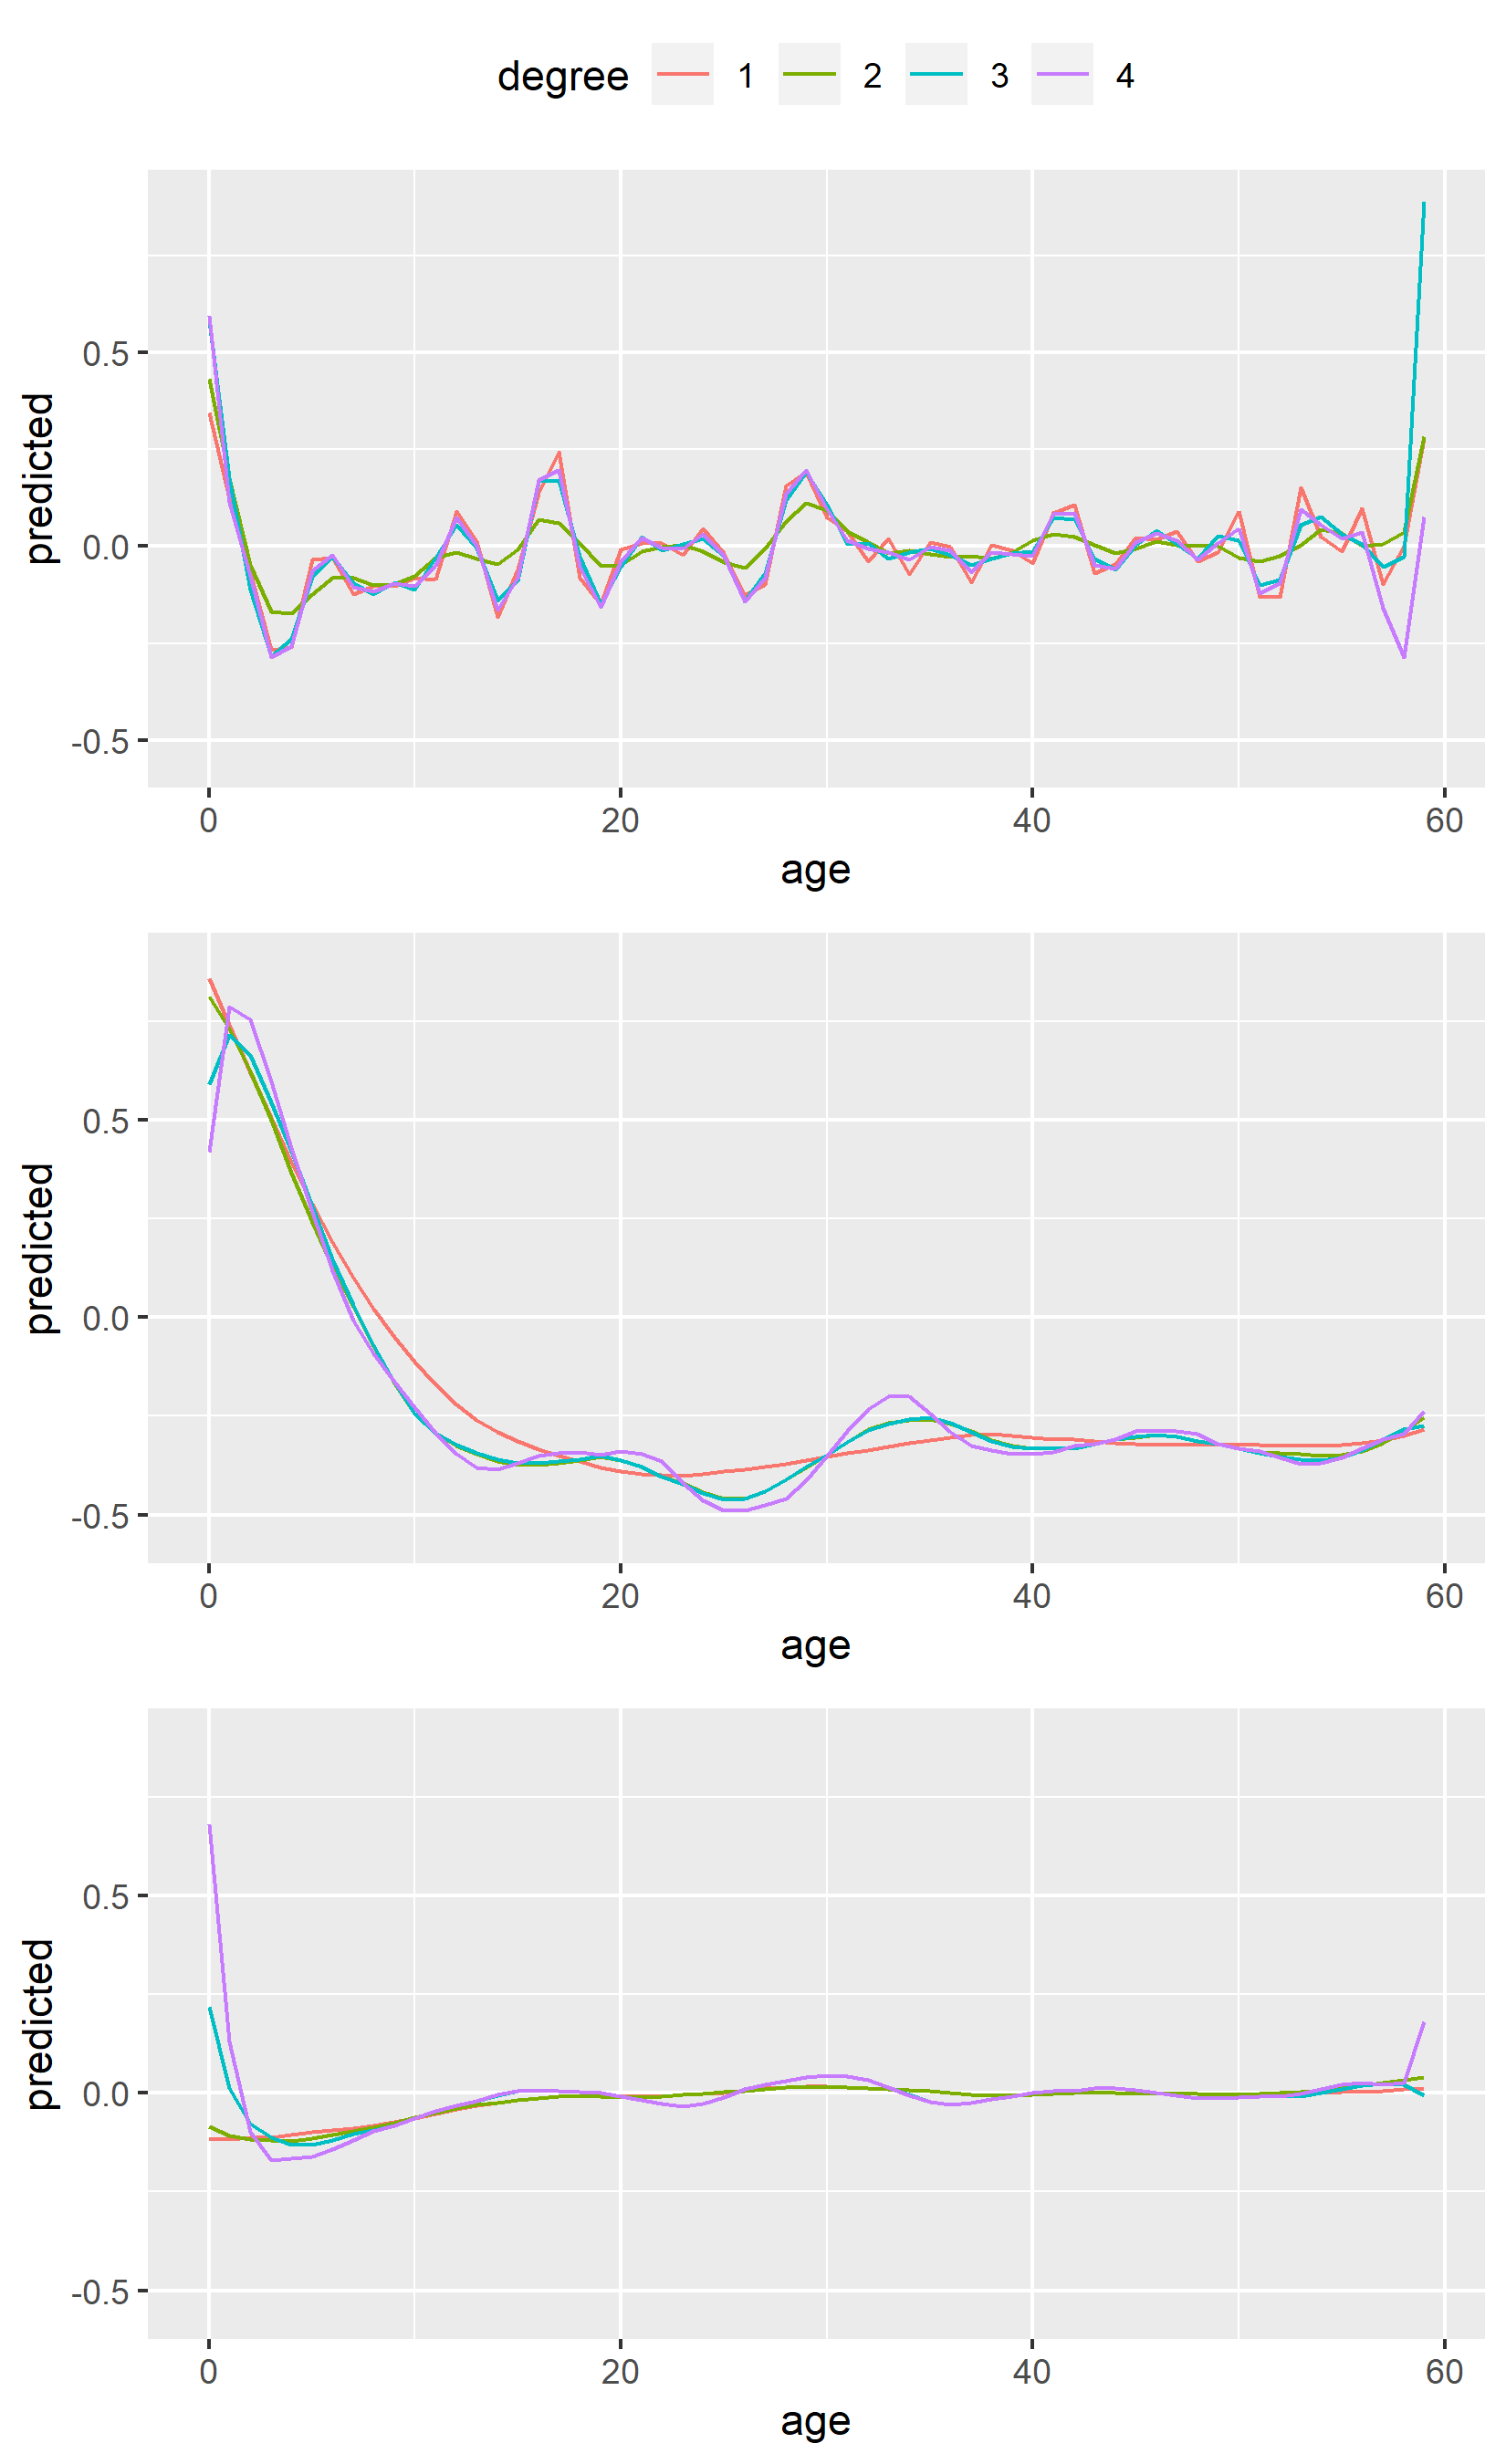
\includegraphics[width=\textwidth, height=0.87\textheight, keepaspectratio]{ex9/deriv.png}
\caption{LPR fits with function \texttt{localpoly.reg} for different polynomial degrees. First plot: first derivative with optimal bandwidths according to \ref{7tableh}; Second plot: regression curve with fixed bandwidth $h=10$; Third plot: first derivative with fixed bandwidth $h=10$.}
\label{7deriv}
\end{figure}

Indeed this function provides all functionality we need for this exercise. The result in the first row Figure \ref{7deriv} show the derivatives with the optimal bandwidths with respect to GCV we found in the last section. We recognize that the strong fluctuation of the regression function itself, shown in the previous section, is also visible for the derivative with is also highly fluctuating and thus in my opinion not really helpful for a reasonable examination of the change in the Z-score. Especially the values at the borders are very high and don't fit at all to the apparently converging behaviour of the data we see in Figure \ref{7fits}. Here we would maybe guess that the Z-score is improving since the derivative is positive but because of the high fluctuation we would expect it to decrease shortly afterwards. I decided to use a higher bandwidth again and fit the curve again (see second and third plot in Figure \ref{7deriv}). I used $h=10$ because it seemed already a reasonable bandwidth in the first section. I included the regression for the actual function and their derivative. Obviously the fluctuation is lower as expected. The fits for degree 3 and 4 still show a slight overfit, especially at the left border. The green and the red line are hard do distinct, so the fit for degree 1 and 2 are very similar. Both start with a negative derivative that tends to 0 and keeps a slightly positive value then. All in all I would conclude that there is a very small improvement of the Z-score at the age of 2 since the red and green curve are slightly above 0 on the right corner of Figure \ref{7deriv} in the last plot. 
